\section{Metodologia}
Este estudo emprega a Análise de Sobrevivência para modelar o tempo até a ocorrência de um evento de interesse: a recompra de um cliente. A metodologia abrange desde a preparação dos dados até a aplicação e avaliação de modelos estatísticos, utilizando uma abordagem que combina técnicas não-paramétricas e semi-paramétricas.

\subsection{Fonte de Dados e Ferramentas}
Os dados utilizados provêm do conjunto \textit{E-commerce Customer for Behavior Analysis}, disponibilizado na plataforma Kaggle \cite{kaggle_dataset}. Trata-se de um dataset sintético com 250.000 registros, simulando transações de clientes em um ambiente de e-commerce.

\subsection{Tratamento dos Dados}
O conjunto de dados utilizado contém 250.000 registros, representando transações de compra, e é composto por 13 variáveis iniciais. 

Toda a análise foi conduzida na linguagem de programação Python \cite{python_soft}. Para a manipulação e o pré-processamento dos dados, foi utilizada a biblioteca \textit{pandas} \cite{mckinney_pandas}. As visualizações gráficas foram geradas com o auxílio das bibliotecas \textit{matplotlib} e \textit{seaborn}. A modelagem de sobrevivência foi implementada utilizando a biblioteca especializada \textit{lifelines} \cite{davidson_pilon_lifelines}.

\subsection{Pré-processamento e Tratamento dos Dados}
A primeira etapa da análise consistiu na exploração e preparação do conjunto de dados. A Tabela \ref{tab:dicionario_dados} apresenta as variáveis originais e suas respectivas descrições.

\begin{table}[h!]
\centering
\caption{Dicionário de dados com as variáveis utilizadas na análise.}
\label{tab:dicionario_dados}
\begin{tabular}{ll}
\toprule
\textbf{Nome da Coluna} & \textbf{Descrição} \\
\midrule
Customer ID & Identificador numérico único para cada cliente. \\
Purchase Date & Data e hora exatas em que a transação foi realizada. \\
Product Category & Categoria do produto comprado (ex: 'Electronics'). \\
Product Price & Preço de uma única unidade do produto. \\
Quantity & Número de unidades do produto compradas. \\
Total Purchase Amount & Valor total da transação (valor do "carrinho"). \\
Payment Method & Método de pagamento utilizado (ex: 'Credit Card'). \\
Returns & Indica se a compra foi devolvida (1) ou não (0). \\
Age & Idade do cliente. \\
Gender & Gênero do cliente (ex: 'Male', 'Female'). \\
Churn & Indica se o cliente abandonou a plataforma (1) ou não (0). \\
\bottomrule
\end{tabular}
\end{table}
\begin{flushleft}
\footnotesize Fonte: Elaborado pelo autor (2025).
\end{flushleft}

O primeiro passo consistiu na preparação dos dados para a análise. A coluna \texttt{Purchase Date}, que estava em formato de texto (\textit{object}), foi convertida para o tipo \texttt{datetime}, permitindo a manipulação de datas e a ordenação cronológica das transações.

Durante a inspeção inicial, observou-se que as colunas \texttt{Customer Age} e \texttt{Age} eram idênticas, indicando uma redundância. Para evitar multicolinearidade e simplificar o modelo, a coluna \texttt{Customer Age} foi removida.

Um ponto de atenção foi a coluna \texttt{Returns}, que indica se uma compra foi devolvida (1) ou não (0). Esta variável possuía um volume significativo de valores ausentes, correspondendo a 19\% do total de registros. A Figura \ref{fig:returns_antes} ilustra a distribuição dos valores, incluindo os ausentes (NaN).

\begin{figure}[h!]
	\centering
	% Substitua 'distribuicao_returns_antes.png' pelo nome do seu arquivo de imagem
	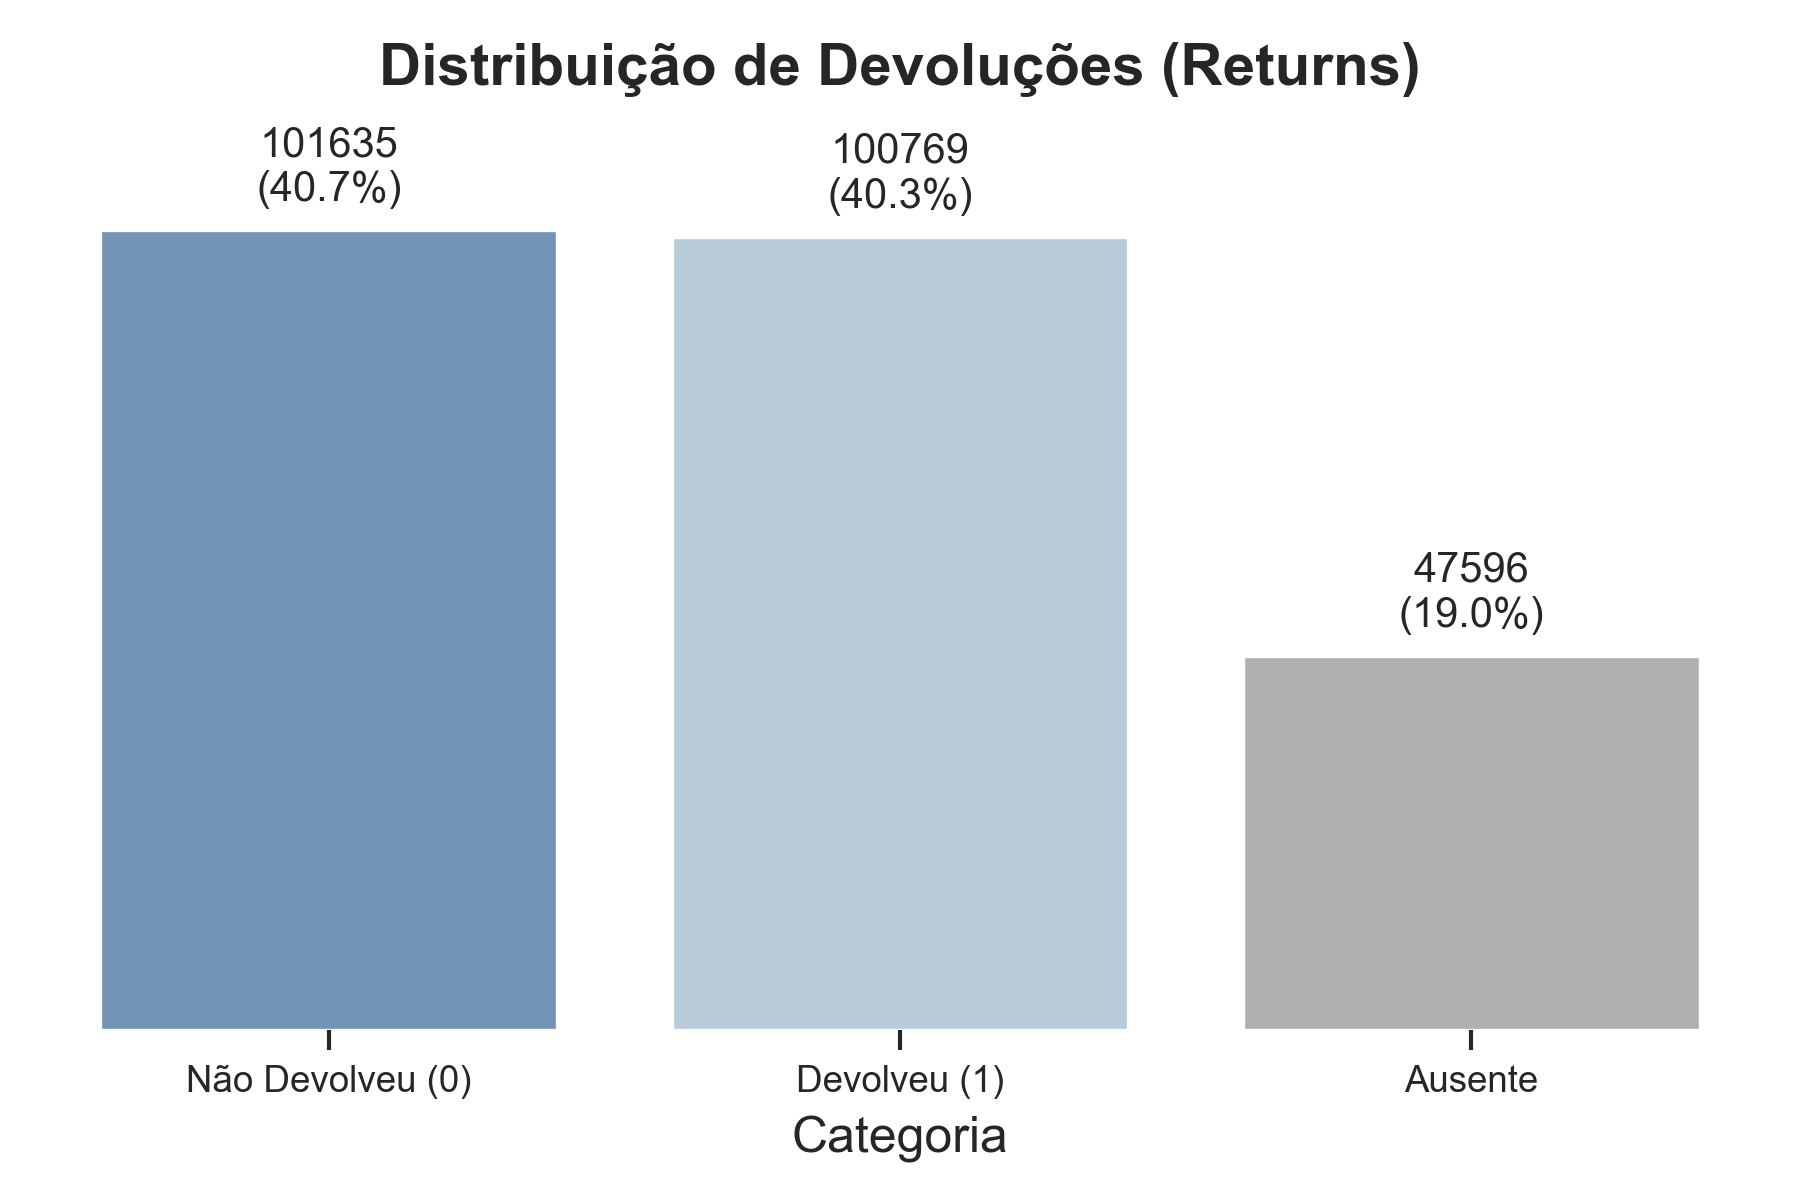
\includegraphics[width=0.7\textwidth]{Imagens/distribuicao_returns_antes.png}
	\caption{Distribuição dos valores da coluna \texttt{Returns} antes do tratamento dos dados ausentes.}
	\label{fig:returns_antes}
\end{figure}
\begin{flushleft}
\footnotesize Fonte: Elaborado pelo autor (2025).
\end{flushleft}

Para o tratamento dos dados faltantes, trabalhou-se com a premissa de que a ausência de um registro de devolução implica que a devolução não ocorreu. Esta é uma abordagem comum quando a documentação do processo de registro de dados não está disponível. Portanto, os valores nulos foram substituídos por 0 (não houve devolução). Após a substituição, a distribuição da variável foi alterada, como pode ser visto na Figura \ref{fig:returns_depois}.

\begin{figure}[h!]
	\centering
	% Substitua 'distribuicao_returns_depois.png' pelo nome do seu arquivo de imagem
	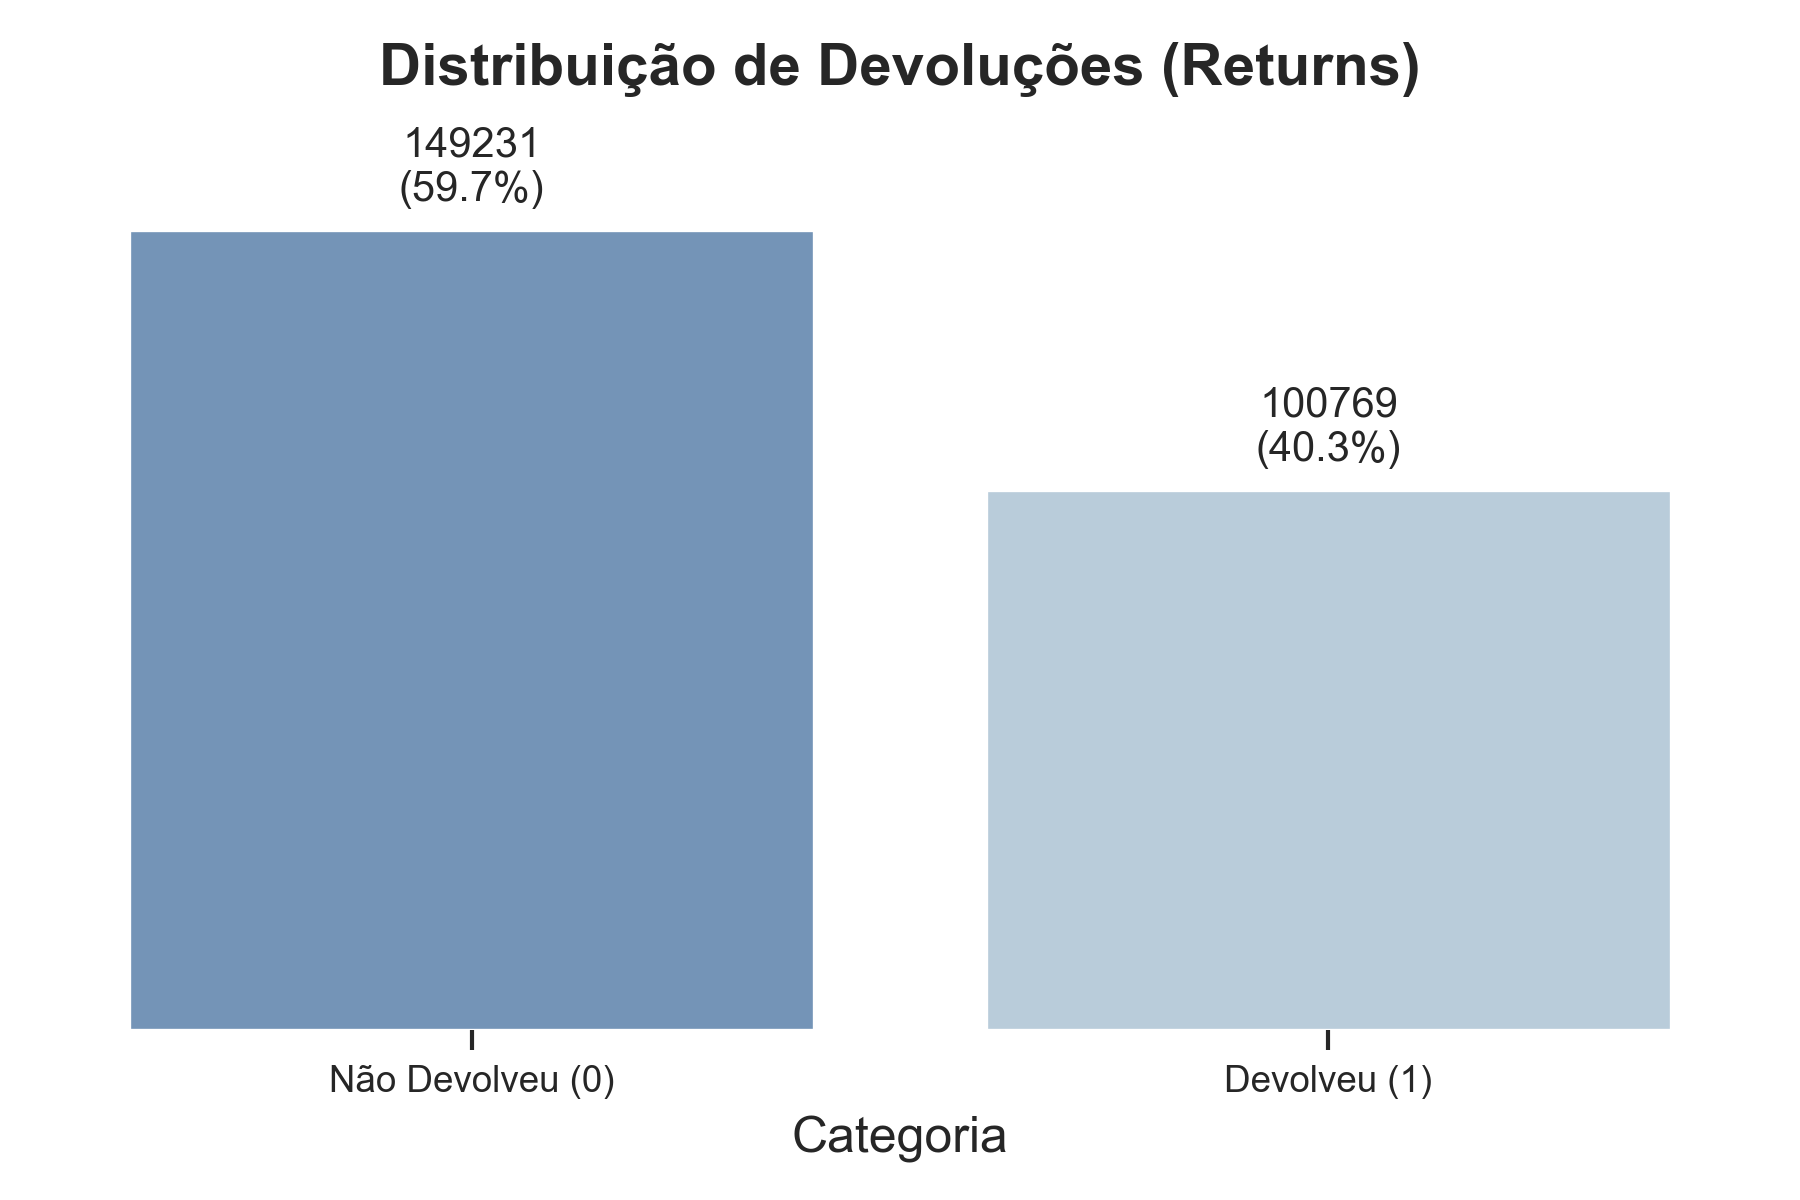
\includegraphics[width=0.7\textwidth]{Imagens/distribuicao_returns_depois.png}
	\caption{Distribuição dos valores da coluna \texttt{Returns} após a substituição de valores nulos por 0.}
	\label{fig:returns_depois}
\end{figure}
\begin{flushleft}
\footnotesize Fonte: Elaborado pelo autor (2025).
\end{flushleft}

\subsection{Engenharia de Atributos para Sobrevivência}
Para aplicar os modelos de sobrevivência, o dataset transacional foi convertido para um formato onde cada linha representa o intervalo entre duas compras consecutivas de um mesmo cliente. Para isso, foram criadas duas variáveis essenciais:
\begin{itemize}
	\item \texttt{duracao}: Representa o tempo (em dias) até o evento. Foi calculada como a diferença entre a data da compra atual e a data da compra seguinte do mesmo cliente.
	\item \texttt{evento}: Uma variável binária indicando a ocorrência do evento de interesse (recompra). Assume o valor 1 se houve uma compra subsequente e 0 caso contrário.
\end{itemize}
Um aspecto fundamental na análise de sobrevivência é o tratamento da \textbf{censura}. Neste estudo, as últimas compras de cada cliente são consideradas dados censurados à direita, pois o evento (recompra) não foi observado até o final do período de estudo. Para esses casos, a \texttt{duracao} foi calculada como o intervalo entre a data da última compra e a data final do estudo (a data mais recente em todo o dataset), e o \texttt{evento} foi definido como 0. A Tabela \ref{tab:exemplo_survival_metodologia} ilustra este processo.

\begin{table}[h!]
\centering
\caption{Exemplo da transformação dos dados para o Cliente ID 46251, ilustrando o cálculo da duração e do evento, incluindo a censura na última observação.}
\label{tab:exemplo_survival_metodologia}
\begin{tabular}{rrrrr}
\hline
\textbf{Customer ID} & \textbf{Purchase Date} & \textbf{proxima\_compra} & \textbf{evento} & \textbf{duracao} \\
\hline
46251 & 2020-09-08 & 2020-11-12 & 1 & 65 \\
46251 & 2020-11-12 & 2022-03-05 & 1 & 477 \\
46251 & 2022-03-05 & 2022-05-23 & 1 & 79 \\
46251 & 2022-05-23 & 2023-09-15 & 0 & 479 \\
\hline
\end{tabular}
\end{table}
\begin{flushleft}
\footnotesize Fonte: Elaborado pelo autor (2025).
\end{flushleft}


\subsection{Modelagem Estatística}
A modelagem estatística foi dividida em duas abordagens complementares: não-paramétrica, para uma análise exploratória robusta das curvas de sobrevivência, e semi-paramétrica, para investigar o efeito de múltiplas covariáveis simultaneamente.

\subsubsection{Métodos Não-Paramétricos}
A abordagem não-paramétrica é fundamental por não impor suposições sobre a distribuição de probabilidade subjacente dos tempos de sobrevivência.

\paragraph{Estimador de Kaplan-Meier}
A primeira técnica utilizada foi o \textbf{Estimador de Kaplan-Meier} \cite{kaplan_meier_1958}, um método para estimar a função de sobrevivência, $S(t)$, a partir de dados que podem ser censurados. A função de sobrevivência representa a probabilidade de um indivíduo (neste caso, o intervalo entre compras de um cliente) "sobreviver" além de um determinado tempo $t$.

O estimador é calculado pela fórmula do produto-limite:
\begin{equation}
\hat{S}(t) = \prod_{i: t_i \le t} \left(1 - \frac{d_i}{n_i}\right)
\end{equation}
Onde:
\begin{itemize}
    \item $t_i$ são os tempos distintos em que pelo menos um evento (recompra) ocorreu.
    \item $d_i$ é o número de eventos que ocorreram no tempo $t_i$.
    \item $n_i$ é o número de indivíduos em risco (clientes cujos intervalos de compra ainda não terminaram ou não foram censurados) imediatamente antes do tempo $t_i$.
\end{itemize}

O resultado é uma curva em degraus, que decresce a cada ocorrência de um evento. A magnitude da queda em cada degrau reflete o risco de evento naquele ponto, condicionado ao número de indivíduos ainda sob observação.

\paragraph{Teste Log-Rank}
Para comparar as curvas de sobrevivência entre dois ou mais grupos (ex: gênero, categoria de produto), foi utilizado o \textbf{teste Log-Rank} \cite{mantel_1966}. Trata-se de um teste de hipóteses não-paramétrico cuja hipótese nula ($H_0$) é que não há diferença entre as funções de sobrevivência dos grupos. A hipótese alternativa ($H_1$) é que pelo menos uma das curvas é diferente das demais.

O teste funciona comparando, em cada tempo de evento $t_i$, o número de eventos observados em cada grupo ($O_{ij}$) com o número de eventos que seriam esperados ($E_{ij}$) se a hipótese nula fosse verdadeira. A estatística do teste é calculada somando as diferenças entre observados e esperados ao longo de todos os tempos de evento, e o resultado segue aproximadamente uma distribuição Qui-quadrado ($\chi^2$) com $k-1$ graus de liberdade, onde $k$ é o número de grupos sendo comparados. A significância é então avaliada a partir do p-valor.

\subsubsection{Métodos Semi-Paramétricos}
\paragraph{Modelo de Riscos Proporcionais de Cox}
Para avaliar o efeito simultâneo de múltiplas covariáveis (tanto numéricas quanto categóricas) sobre o tempo de sobrevivência, foi empregado o \textbf{Modelo de Riscos Proporcionais de Cox} \cite{cox_1972}. Este é um modelo de regressão semi-paramétrico que modela a função de risco (ou taxa de falha), $h(t)$, que representa o risco instantâneo de um evento ocorrer no tempo $t$, dado que o indivíduo sobreviveu até aquele momento.

A fórmula do modelo de Cox é:
\begin{equation}
h(t | \mathbf{X}) = h_0(t) \exp(\beta_1 X_1 + \beta_2 X_2 + \dots + \beta_p X_p) = h_0(t) \exp(\mathbf{X}\boldsymbol{\beta})
\end{equation}
Onde:
\begin{itemize}
    \item $h(t | \mathbf{X})$ é a função de risco no tempo $t$ para um indivíduo com um vetor de covariáveis $\mathbf{X}$.
    \item $h_0(t)$ é a função de risco base (\textit{baseline hazard}), que é a parte não-paramétrica do modelo. Ela representa o risco quando todas as covariáveis são zero e não precisa ser especificada para a estimação dos coeficientes.
    \item $\mathbf{X} = (X_1, X_2, \dots, X_p)$ é o vetor de covariáveis para o indivíduo.
    \item $\boldsymbol{\beta} = (\beta_1, \beta_2, \dots, \beta_p)$ é o vetor de coeficientes de regressão, estimados a partir dos dados através de máxima verossimilhança parcial.
\end{itemize}
O resultado principal do modelo é a \textbf{Razão de Riscos} (\textit{Hazard Ratio}, HR), calculada como $\exp(\beta_i)$. Um HR > 1 para uma covariável indica que um aumento na mesma está associado a um maior risco de ocorrência do evento, enquanto um HR < 1 indica um menor risco. O modelo se baseia na premissa de \textit{riscos proporcionais}, que assume que o efeito das covariáveis sobre o risco é constante ao longo do tempo.

\subsection{Avaliação dos Modelos}
A validação e comparação dos modelos foram realizadas com métricas apropriadas para cada técnica. Para o teste Log-Rank, a significância estatística foi avaliada com base no p-valor, utilizando um nível de significância de $\alpha = 0.05$.

O desempenho do modelo de Cox foi avaliado utilizando o \textbf{Índice de Concordância (C-index)} \cite{harrell_1982}. Esta métrica avalia a capacidade discriminatória do modelo, sendo análoga à Área Sob a Curva ROC (AUC) em modelos de classificação. O C-index mede a proporção de todos os pares de indivíduos possíveis em que o modelo prediz corretamente a ordem dos seus tempos de sobrevivência. Especificamente, de todos os pares em que um indivíduo teve o evento antes do outro, qual a proporção em que o indivíduo com o menor tempo de sobrevivência previsto de fato teve o evento primeiro. Um valor de 0.5 indica um desempenho aleatório, enquanto 1.0 representa uma predição perfeita.
